% --------------------------------------------------------------------------
% Version 3.0
% This template is available on the sites:
% https://www.overleaf.com/read/rpkkfchcnbsc
% https://www.overleaf.com/latex/templates/itmo-beamer-theme/fpttrgnmqwsb
% https://github.com/AlexZabashta/ITMO-Beamer-theme
% --------------------------------------------------------------------------

% Attention!!!
% This document was created only as an example of using ITMO beamer styling.
% Don't use it as a Latex or beamer tutorial!
% Check out the capabilities of Latex and beamer (at least basic) independently.


\documentclass[aspectratio=169]{beamer}
\usepackage{ITMOtheme}
\setbeamercovered{dynamic}

\usepackage{tikz}
\usepackage{pgfplots}
\pgfplotsset{compat=1.18}

% Use this package to automatically format references.
% \usepackage[style=mla]{biblatex}
% \addbibresource{references.bib}



% The fields 'title', 'author', 'subject', 'keywords' are used to generate a PDF document.
% It is recommended that you fill them in, even if you are creating your title slide manually.

% use \title[short title]{full title}
\title[ITMO LaTex]{ITMO University LaTex Presentation}

%\subtitle[short subtitle]{long subtitle}

\author[LastName F.]{FirstName LastName}

%\institute[short institute]{long institute}

\where{St. Petersburg}
\date{\today}


\subject{example}
\keywords{ITMO University, LaTex teamplate, beamer}



\begin{document}

% Title slide
\begin{frame}[plain,noframenumbering]
    \itmobackgroundsnakes{
        \vfill
        \begin{center}
            \vspace{2cm}
            
            {\usebeamerfont{title}\LARGE\textbf{``The Game Beneath the Game:\\The Evolution of Cheats and Anti-Cheat Systems in Counter-Strike 2''}}\\[1.5em]
            
            \textbf{Author:} Pablo Valiente\\[0.5em]
            \textbf{Supervisor:} Dr. Antonio Nappa\\[3em]
            \textbf{Universidad Carlos III de Madrid}\\[1em]
            \textbf{Academic Year:} 2024--2025\\[0.5em]
        \end{center}
        \vfill
    }
\end{frame}

% Table of Contents slide
\begin{frame}[plain,noframenumbering]
    \frametitle{Table of Contents}
    \Large
    \begin{enumerate}
        \item Motivation and Context
        \pause
        \item Cheating: History, Ecosystem, and Ethics
        \pause
        \item Anti-Cheat Technologies and Milestones
        \pause
        \item Case Study: Counter-Strike 2
        \pause
        \item Technical Analysis: Injection and Evasion
        \pause
        \item Game Logic Manipulation and Visual Features
        \pause
        \item Final Reflections and Future Directions
    \end{enumerate}
\end{frame}

% --- Motivation and Context ---
\section{Motivation and Context}
\begin{frame}
    \frametitle{Motivation}
    My interest in this topic began around six years ago, driven by a passion for competitive video games.
    \vspace{0.4cm}
    \begin{itemize}
        \item \textbf{Curiosity:} Encountering cheaters in ranked matches often led me to wonder: \textit{“How did they do it?”}
        \pause
        \item \textbf{Exploration:} This question gradually introduced me to reverse engineering, memory analysis, and anti-cheat evasion.
        \pause
        \item \textbf{Background:} Over the years, I acquired technical knowledge through communities, experiments, and academic training.
        \pause
        \item \textbf{Objective:} To merge this journey with a rigorous academic study by analyzing and implementing real cheats to test detection systems.
    \end{itemize}
\end{frame}

% --- Added thesis sections and slides ---

\AtBeginSection[]{
    \begin{frame}
        \frametitle{Outline}
        \tableofcontents[
            currentsection,
            sectionstyle=show/shaded,
            hideothersubsections
        ]
    \end{frame}
}



% --- New Introductory Slides: Cheating Phenomenon ---

% --- Cheating: History, Ecosystem, and Ethics ---
\section{The Evolution of Cheating: History, Ecosystem, and Ethics}
\begin{frame}
    \frametitle{Understanding Cheating in Online Games}
    Cheating undermines fairness and security in competitive online games.
    \vspace{0.4cm}
    \begin{itemize}
        \item \textbf{Definition:} Any software or hardware manipulation that grants unfair advantage.
        \pause
        \item \textbf{Anti-Cheat:} Monitors and enforces integrity at runtime, acting like an \textbf{EDR} by detecting anomalous behavior, unauthorized memory access, or code injection in protected processes.
        \pause
        \item \textbf{Spectrum:} From basic aimbots to advanced GUI Drawings.
        \pause
        \item \textbf{Impact:} Threatens matchmaking integrity and industry revenue.
        \pause
        \item \textbf{Context:} Now part of the broader cybersecurity landscape.
    \end{itemize}
\end{frame}

\begin{frame}
    \frametitle{Origins of Cheating: From Debugging to Subversion}
    Cheating emerged from tools meant for testing and evolved into manipulation.
    \vspace{0.4cm}
    \begin{itemize}
        \item \textbf{Debug Codes:} Became public cheat codes (e.g., Konami Code).
        \pause
        \item \textbf{GameShark:} Modified RAM directly on console hardware.
        \pause
        \item \textbf{Cheat Engine:} Enabled runtime memory editing on PC.
        \pause
        \item \textbf{x64dbg and ReClass.NET:} Allowed advanced memory mapping, pointer tracing, and class reconstruction.
        \pause
        \item \textbf{Advanced Tooling:} Debuggers like \texttt{x64dbg}, memory editors, and tools such as \texttt{ReClass.NET} enabled deep inspection of structures and dynamic memory regions.
    \end{itemize}
\end{frame}

\begin{frame}
    \frametitle{From Hacks to Services: The Turning Point}
    The early 2010s marked a major shift in how cheats were created, distributed, and perceived.
    \vspace{0.4cm}
    \begin{itemize}
        \item \textbf{Community Forums:} Platforms like UnKnoWnCheaTs fostered knowledge sharing and tutorials.
        \pause
        \item \textbf{Toolchains:} Public tools and open-source loaders lowered the barrier to entry.
        \pause
        \item \textbf{Subscription Models:} Private cheats became commercialized with regular updates and support.
        \pause
        \item \textbf{User Demand:} Players sought not just to win, but to dominate with minimal effort, fueling a sustainable market.
    \end{itemize}
\end{frame}

\begin{frame}
    \frametitle{Cheating Today: A Professionalized Ecosystem}
    Cheating has evolved from hobbyist tools to a mature ecosystem that mirrors legitimate software development.
    \vspace{0.4cm}
    \begin{itemize}
        \item \textbf{Commercialization:} Cheat providers operate like startups, offering licensing, tiered features, and customer support.
        \pause
        \item \textbf{Stealth Technology:} Use of polymorphism, virtualization, and driver-level code to evade detection.
        \pause
        \item \textbf{Infrastructure:} Loaders, obfuscators, HWID spoofers, and encrypted update channels ensure persistence.
        \pause
        \item \textbf{Community:} Development is sustained by highly technical reverse engineers who are constantly reversing every update in the game.
    \end{itemize}
\end{frame}


% --- Anti-Cheat Timeline Table ---
% --- Anti-Cheat Technologies and Milestones ---
\section{The Rise of Anti-Cheat: Technologies and Milestones}
\begin{frame}
    \frametitle{Anti-Cheat Systems Timeline}
    Anti-cheat systems have evolved from basic client-side tools to complex, kernel-level detectors. Each marked a significant shift in visibility, access, or enforcement.
    \vspace{0.4cm}
    \begin{table}[]
        \small
        \begin{tabular}{|l|l|l|l|}
            \hline
            \textbf{System} & \textbf{Year} & \textbf{Mode} & \textbf{Milestone or Innovation} \\
            \hline
            PunkBuster & 2000 & User & First real-time memory scan and screenshot system \\
            VAC & 2002 & User & Delayed ban model to obfuscate detection methods \\
            BattleEye & 2004 & Kernel & Early adoption of kernel-mode drivers \\
            FairFight & 2012 & Server & Behavioral/statistical detection at server level \\
            EAC & 2018 & Kernel & Real-time scanning with driver-level protection \\
            Vanguard & 2020 & Kernel & Persistent always-on kernel driver (controversial) \\
            VAC Live & 2023 & Hybrid & Real-time detection with low-latency enforcement \\
            \hline
        \end{tabular}
    \end{table}
\end{frame}

% --- NEW: Genre-Specific Vulnerabilities Slide ---
\begin{frame}
    \frametitle{Why FPS Games Are Especially Vulnerable}
    First-person shooters present unique architectural weaknesses that make them highly susceptible to game manipulation.
    \vspace{0.4cm}
    \begin{itemize}
        \item \textbf{Client-Side Rendering:} The game client must access enemy positions to render them, even through walls.
        \pause
        \item \textbf{Memory Residency:} Positional and player state data exist in memory and can be externally read or modified.
        \pause
        \item \textbf{Contrast With Strategy Games:} RTS or turn-based titles store game logic server-side, making manipulation far more difficult.
        \pause
        \item \textbf{Exploitation Vector:} These FPS traits enable features like ESP, aimbots, and recoil control by hijacking user input or memory data.
    \end{itemize}
\end{frame}



% --- Justification Slide: Why Counter-Strike 2? ---
\begin{frame}
    \frametitle{Why Counter-Strike 2?}
    Counter-Strike 2 represents a prime environment to study modern cheating.
    \vspace{0.4cm}
    \begin{itemize}
        \item \textbf{Large Player Base:} Over 1 million monthly active users in 2024--2025.
        \pause
        \item \textbf{High Competitive Stakes:} Ranked ladders, esports scene, and skin economy intensify incentives.
        \pause
        \item \textbf{Persistent Cheating Problem:} VAC bans, report abuse, and public complaints highlight widespread issues.
        \pause
        \item \textbf{Technical Maturity:} CS2 is built on Source 2 with new anti-cheat features and detection paradigms.
        \pause
        \item \textbf{Public Data:} Rich dataset from platforms like SteamCharts and CSStats enables evidence-based analysis.
    \end{itemize}
\end{frame}




% --- NEW: CS2 Player Base Growth Slide ---
\begin{frame}
    \frametitle{CS2 Player Base Growth (2024–2025)}
    To contextualize the scale of CS2's ecosystem, the following graph illustrates the evolution of its player base based on SteamCharts data.
    \vspace{0.3cm}
    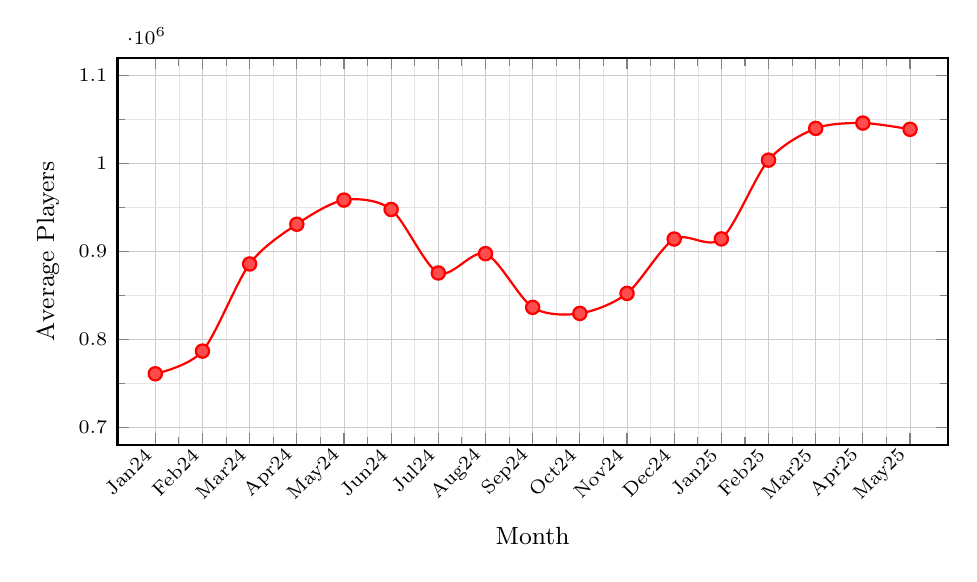
\begin{tikzpicture}
    \begin{axis}[
        width=\linewidth,
        height=6.5cm,
        xlabel={Month},
        ylabel={Average Players},
        symbolic x coords={Jan24, Feb24, Mar24, Apr24, May24, Jun24, Jul24, Aug24, Sep24, Oct24, Nov24, Dec24, Jan25, Feb25, Mar25, Apr25, May25},
        xtick=data,
        xticklabel style={rotate=45, anchor=east, font=\scriptsize},
        yticklabel style={font=\scriptsize},
        label style={font=\small},
        tick style={thin},
        grid=both,
        minor tick num=1,
        major grid style={line width=.3pt, draw=gray!40},
        minor grid style={line width=.2pt, draw=gray!20},
        ymin=700000, ymax=1100000,
        enlargelimits=0.05,
        smooth,
        mark options={scale=1.2, fill=red!70},
        line width=0.8pt,
        legend style={at={(0.5,-0.2)}, anchor=north, font=\small},
    ]
    \addplot[
        color=red,
        mark=*,
    ]
    coordinates {
        (Jan24,760859) (Feb24,786631) (Mar24,885630) (Apr24,930749)
        (May24,958207) (Jun24,947521) (Jul24,875365) (Aug24,897338)
        (Sep24,836307) (Oct24,829439) (Nov24,852164) (Dec24,913953)
        (Jan25,914092) (Feb25,1003571) (Mar25,1039663) (Apr25,1045702)
        (May25,1038597)
    };
    \end{axis}
    \end{tikzpicture}
\end{frame}

% --- NEW: Steam Top 10 Visual Context Slide ---
\begin{frame}
    \frametitle{Steam Top 10: July 7, 2025}
    \begin{center}
        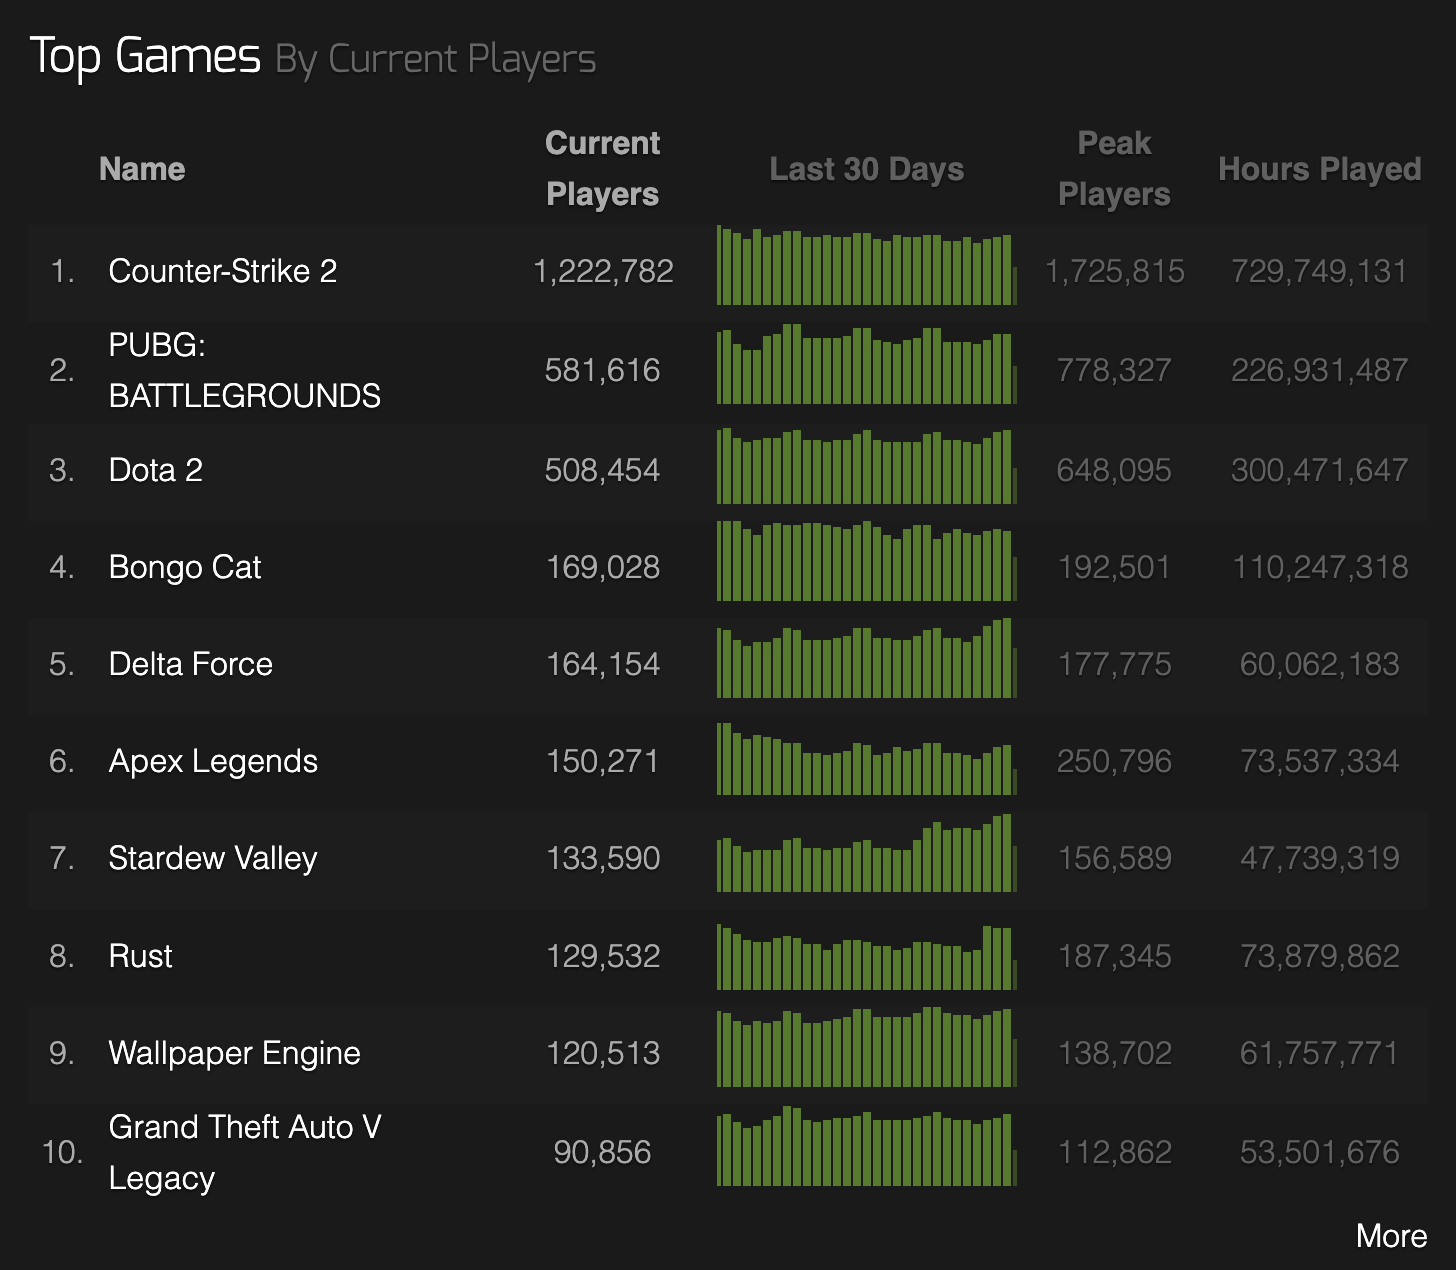
\includegraphics[width=0.63\linewidth]{images/steam_stats.png}
    \end{center}
    \vspace{0.3cm}
\end{frame}

\section{Counter-Strike 2: A Case Study in Cheating Dynamics}

% --- NEW: VAC Anti-Cheat Strategy Slide ---
\begin{frame}
    \frametitle{VAC: Valve's Anti-Cheat Strategy}
    Since the early days of Counter-Strike, Valve has maintained its own anti-cheat system, VAC (Valve Anti-Cheat).
    \vspace{0.4cm}
    \begin{itemize}
        \item \textbf{Consistency:} VAC has been used since CS 1.6 and evolved alongside the series.
        \pause
        \item \textbf{User Mode Limitation:} VAC operates entirely in user space, unlike newer kernel-mode anticheats.
        \pause
        \item \textbf{Detection Philosophy:} Prefers silent detection with delayed banwaves to avoid tipping off cheat developers.
        \pause
        \item \textbf{Upcoming Evolution:} Valve announced integration of \textbf{machine learning models} into VAC Live to detect behavioral patterns and cheating heuristics in real time.
    \end{itemize}
\end{frame}


% --- Improved Trust Factor and Detection Challenges ---
\begin{frame}
    \frametitle{Trust Factor and Detection Challenges}
    Valve's Trust Factor system, introduced in late 2017, fundamentally changed matchmaking by leveraging a hidden reputation metric to segregate players. 
    \vspace{0.4cm}
    \begin{itemize}
        \item \textbf{Function:} Uses behavioral data, report history, account characteristics, and system metrics to infer player reliability.
        \pause
        \item \textbf{Segregation Strategy:} Groups suspect cheaters with other suspect cheaters, and legitimate players with each other, to reduce disruptive overlap.
        \pause
        \item \textbf{Opacity:} The exact calculation is hidden, preventing transparency or dispute of unfair evaluations.
    \end{itemize}
\end{frame}

% --- NEW: What Actually Affects Trust Factor? ---
\begin{frame}
    \frametitle{What Actually Affects Trust Factor?}
    Although Valve keeps the exact algorithm secret, several factors are known or strongly suspected to influence Trust Factor:
    \vspace{0.4cm}
    \begin{itemize}
        \item \textbf{Account Age and Game Hours:} Older accounts and higher total playtime positively impact Trust Factor.
        \pause
        \item \textbf{Money Spent:} Purchasing games or items (e.g., skins, Prime status) improves account reputation.
        \pause
        \item \textbf{Report History:} Frequent reports, especially confirmed ones, lower your Trust Factor.
        \pause
        \item \textbf{Friend Network:} Being friends with banned or suspicious players may reduce your Trust Factor.
    \end{itemize}
\end{frame}

% --- Improved Economic and Psychological Impact ---
\begin{frame}
    \frametitle{Economic and Psychological Impact}
    Cheating in CS2 generates profound economic losses and undermines player well-being.
    \vspace{0.4cm}
    \begin{itemize}
        \item \textbf{Skin Markets:} \textbf{VAC bans} can instantly invalidate cosmetic items worth \textbf{thousands of euros}. Locking down those accounts and disabling trade offers.
        \pause
        \item \textbf{Morale:} \textbf{Rampant cheating} erodes competitive spirit, trust, and perceived fairness.
        \pause
        \item \textbf{Retention:} \textbf{Frustrated players} abandon the game, shrinking and destabilizing the community.
    \end{itemize}
\end{frame}

% --- NEW: Survey Slide: Cheating as a Critical Threat ---
\begin{frame}
    \frametitle{Survey: Cheating as a Critical Threat}
    A 2018 global survey by Irdeto revealed the widespread negative impact of cheating in Counter-Strike: Global Offensive:
    \vspace{0.4cm}
    \begin{table}[]
        \small
        \centering
        \begin{tabular}{|p{7.5cm}|c|}
            \hline
            \textbf{Survey Statement} & \textbf{Percentage} \\
            \hline
            Experienced negative impact due to cheating  & 60\% \\
            \hline
            Would stop playing a game because of cheaters & 77\% \\
            \hline
            Support permanent bans for cheaters & 69\% \\
            \hline
            Believe developers are not doing enough & 55\% \\
            \hline
        \end{tabular}
    \end{table}
    \vspace{0.2cm}
    \begin{itemize}
        \item Highlights long-term damage to player trust and retention.
        \item Economic implications due to reduced engagement and spending.
    \end{itemize}
\end{frame}

% --- Quantitative Data Analysis Slide (NEW) ---
\begin{frame}
    \frametitle{Quantifying the Impact: Cheating and Player Statistics}
    Beyond anecdotal evidence, empirical data helps us understand the scope of cheating in CS2.
    \vspace{0.4cm}
    \begin{itemize}
        \item \textbf{Player Growth:} Monthly average players increased from 760k to over 1 million (SteamCharts, Jan 2024 -- May 2025).
        \pause
        \item \textbf{Delayed Enforcement:} 28\% of VAC bans occur within 24h of last match; average delay is 20 days.
        \pause
        \item \textbf{Cheating Embedded:} 97\% of affected matches had only one banned player, often undetected in real time.
        \pause
        \item \textbf{No Case Farming Evidence:} Cheaters are not primarily motivated by item drops but by gameplay disruption or rank inflation.
    \end{itemize}
\end{frame}


\section{Code Injection and Cheat Delivery Mechanisms}

\begin{frame}
    \frametitle{DLL Injection and Manual Mapping}
    Cheats are commonly implemented as DLL files injected into the game process.
    \vspace{0.4cm}
    \begin{itemize}
        \item \textbf{Classic Methods:} LoadLibrary and CreateRemoteThread are frequently used, but easily detected.
        \pause
        \item \textbf{Manual Mapping:} Avoids standard API calls, skipping LoadLibrary and not registering the module.
        \pause
        \item \textbf{Stealth Advantage:} Enables loading cheat code directly into memory without leaving traces.
        \pause
        \item \textbf{Malware Parallels:} These techniques mirror malware behavior, stealthy, evasive, and persistent.
    \end{itemize}
\end{frame}

\begin{frame}
    \frametitle{Real-World Implementation: Cheat Loaders}
    Modern cheat providers rely on custom loaders rather than directly sharing raw DLLs.
    \vspace{0.4cm}
    \begin{itemize}
        \item \textbf{Encrypted Payloads:} DLLs are downloaded and decrypted at runtime.
        \pause
        \item \textbf{Anti-Detection Techniques:} Loaders bypass anti-cheat hooks and spoof return addresses.
        \pause
        \item \textbf{Examples:} Popular cheats like \textit{NeverLose} and \textit{Skeet} deploy secure loaders to ensure stealth.
        \pause
        \item \textbf{Operational Flow:}\\
    \vspace{0.6cm}
    \begin{center}
        \texttt{Launch loader → Restart Steam → Inject payload → Execute entry point silently}
    \end{center}
    \end{itemize}
\end{frame}

\begin{frame}
    \frametitle{VAC Detection and Countermeasures}
    VAC employs traditional and modern detection mechanisms to identify unauthorized modifications.
    \vspace{0.4cm}
    \begin{itemize}
        \item \textbf{Detection Vectors:} Includes signature scanning, suspicious thread start addresses, and VMT hook detection.
        \pause
        \item \textbf{Reversing Insight:} Analyzing \texttt{steamservice.dll} reveals that VAC streams detection modules from Valve servers.
        \pause
        \item \textbf{PE Injection:} These modules are manually mapped into memory using PE Injection.
        \pause
        \item \textbf{Dynamic Landscape:} The result is a constant arms race between detection systems and cheat developers.
    \end{itemize}
\end{frame}

\section{Cheat Implementation: Hooking, Logic, and Features}

\begin{frame}
    \frametitle{Hooking the Engine: Input, Rendering, and Events}
    Hooking allows interception of internal engine calls to alter behavior at runtime.
    \vspace{0.4cm}
    \begin{itemize}
        \item \textbf{Initial Step:} Reverse engineer the game binary to locate key virtual functions related to input, rendering, or entity updates.
        \pause
        \item \textbf{Hooking Layer:} Inject trampoline hooks to redirect control flow to our cheat-defined functions.
        \pause
        \item \textbf{MinHook Library:} We employed \texttt{MinHook} for ease of use and reliability.
        \pause
        \item \textbf{Limitations:} While MinHook is sufficient for prototyping, more stealth-oriented alternatives exist (e.g., Shadow Hooking, Page Guard, or VEH-based hooks).
    \end{itemize}
\end{frame}

% --- Improved Entity List and Memory Traversal Slide ---
\begin{frame}
    \frametitle{Entity List and Memory Traversal}
    During the reverse engineering process of CS2, we identified how entities are registered and updated in memory.
    \vspace{0.4cm}
    \begin{itemize}
        \item \textbf{Entity Management:} The game uses a handle-based paging system to manage all in-game entities.
        \pause
        \item \textbf{Callback Hooks:} We named the functions \texttt{OnAddEntity} and \texttt{OnRemoveEntity} during our reverse engineering, as they lack debug symbols. These routines are ideal hook points to track player spawns and despawns.
        \pause
        \item \textbf{Memory Structures:} Reverse engineering revealed a central list containing pointers to entity classes and their data.
    \end{itemize}
\end{frame}

% --- NEW: Implementation of Cheat Features Slide ---
\begin{frame}
    \frametitle{From Theory to Practice: Implementing Cheat Features}
    Once the game’s memory structures and entity management system are fully understood, the implementation of cheat features becomes straightforward.
    \vspace{0.4cm}
    \begin{itemize}
        \item \textbf{Features Developed:}
        \begin{itemize}
            \item \textit{Chams}: custom materials to highlight player models through geometry.
            \pause
            \item \textit{Aimbot}: automatic aim adjustment based on enemy position, using directional vector math and angle normalization (see equations in appendix).
            \pause
            \item \textit{Bunny Hop (BHop)}: automated jump timing to maximize movement speed.
            \pause
            \item \textit{Visual Enhancements}: overlays and tweaks to highlight relevant data in the scene.
            \pause
            \item \textit{Bone ESP}: skeletal rendering of player models to track posture and positioning through obstacles.
        \end{itemize}
    \end{itemize}
\end{frame}



% (section absorbed in previous title, line removed)


\begin{frame}
    \frametitle{Chams: Internal Material Injection}
    To implement Chams, we reverse engineered one of CS2’s internal material files to understand its structure.
    \vspace{0.4cm}
    \begin{itemize}
        \item \textbf{Material Discovery:} We decrypted and analyzed a material from Valve's asset system (suspected format: \texttt{.vk3}).
        \pause
        \item \textbf{Material Creation:} This allowed us to mimic and reconstruct materials programmatically.
        \pause
        \item \textbf{Function Hooks:} We hooked two internal engine functions: one responsible for material creation, another for rendering passes.
        \pause
        \item \textbf{Selective Injection:} By filtering the render queue, we applied our custom material only to specific models (e.g., player entities, weapons).
        \pause
        \item \textbf{Outcome:} Player models become visually enhanced through walls using internal rendering only.
    \end{itemize}
\end{frame}

% --- Visual Examples: Chams Materials ---
\begin{frame}
    \frametitle{Visual Examples: Chams Materials}        
    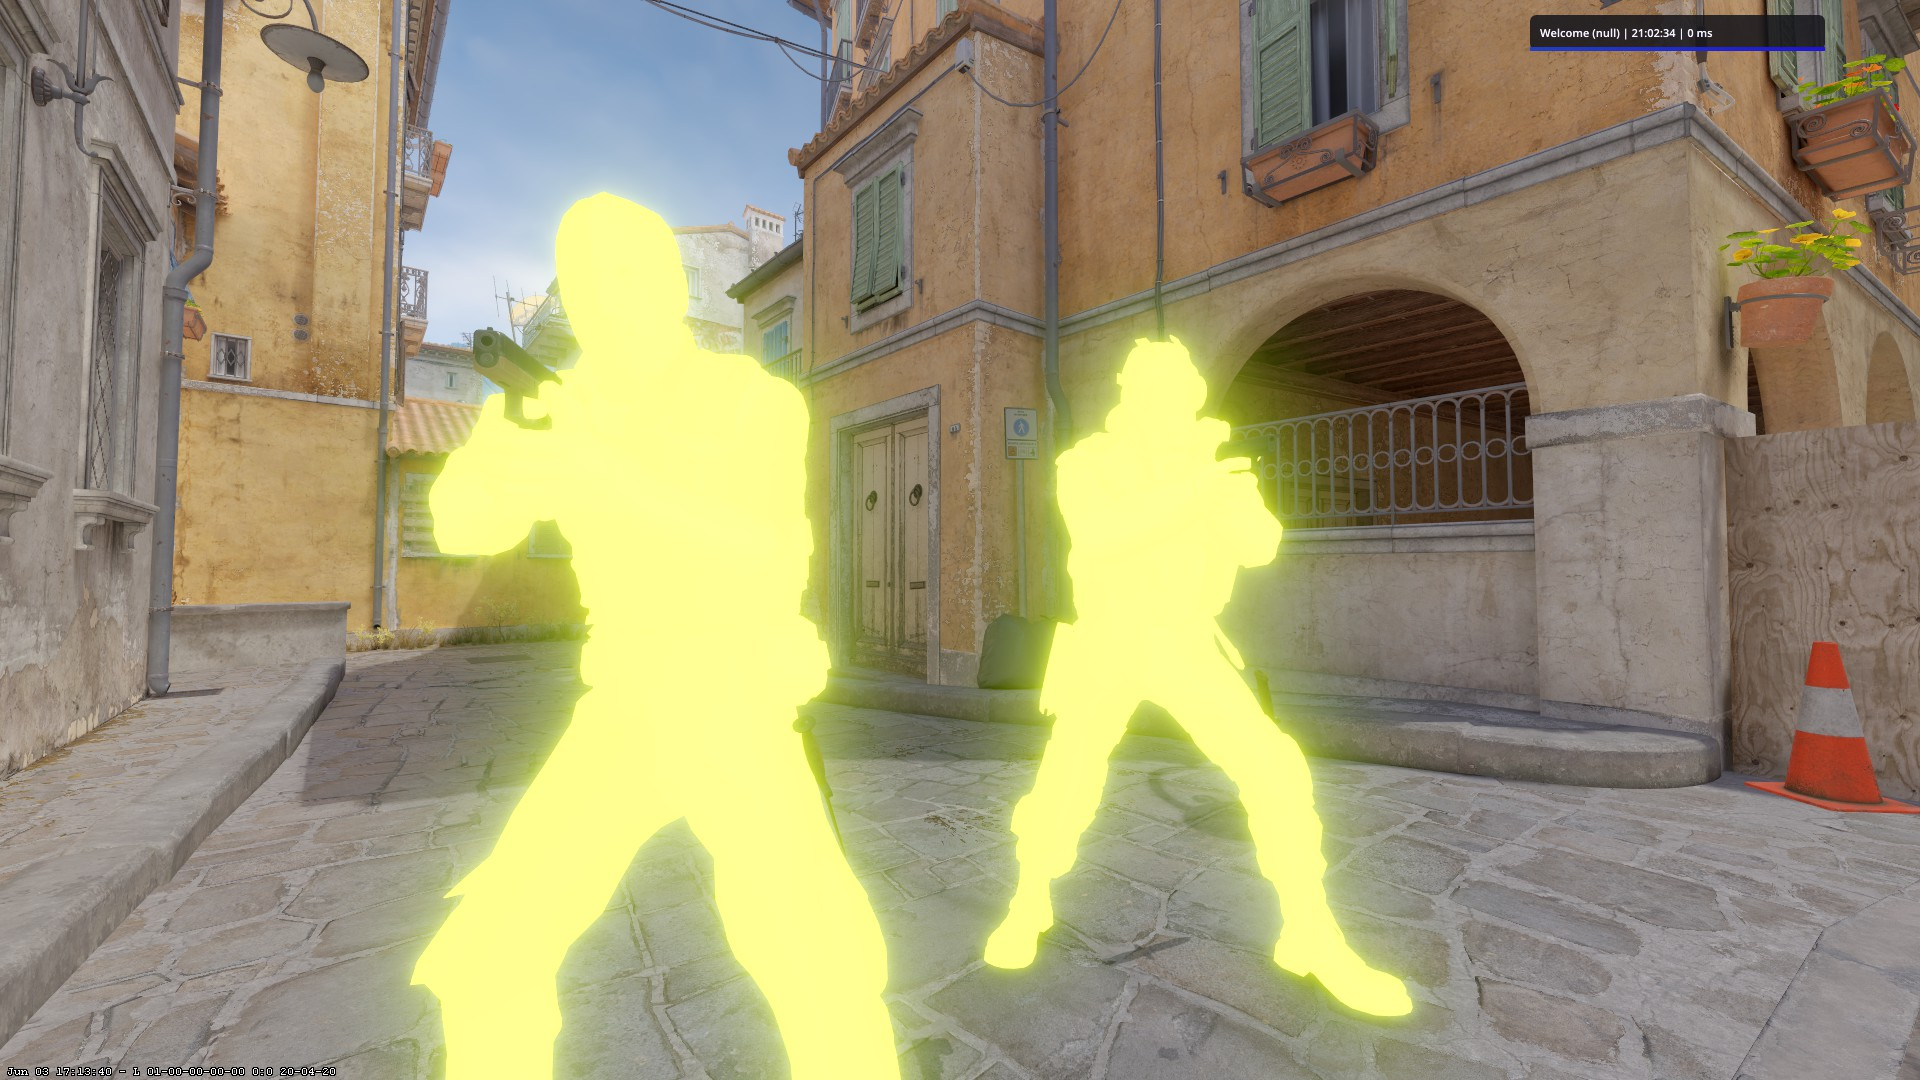
\includegraphics[width=1\linewidth]{../Master Thesis Template/images/chams/chams_demo/20250608210234_1.jpg}
\end{frame}

\begin{frame}
    \frametitle{Visual Examples: Chams Materials}        
    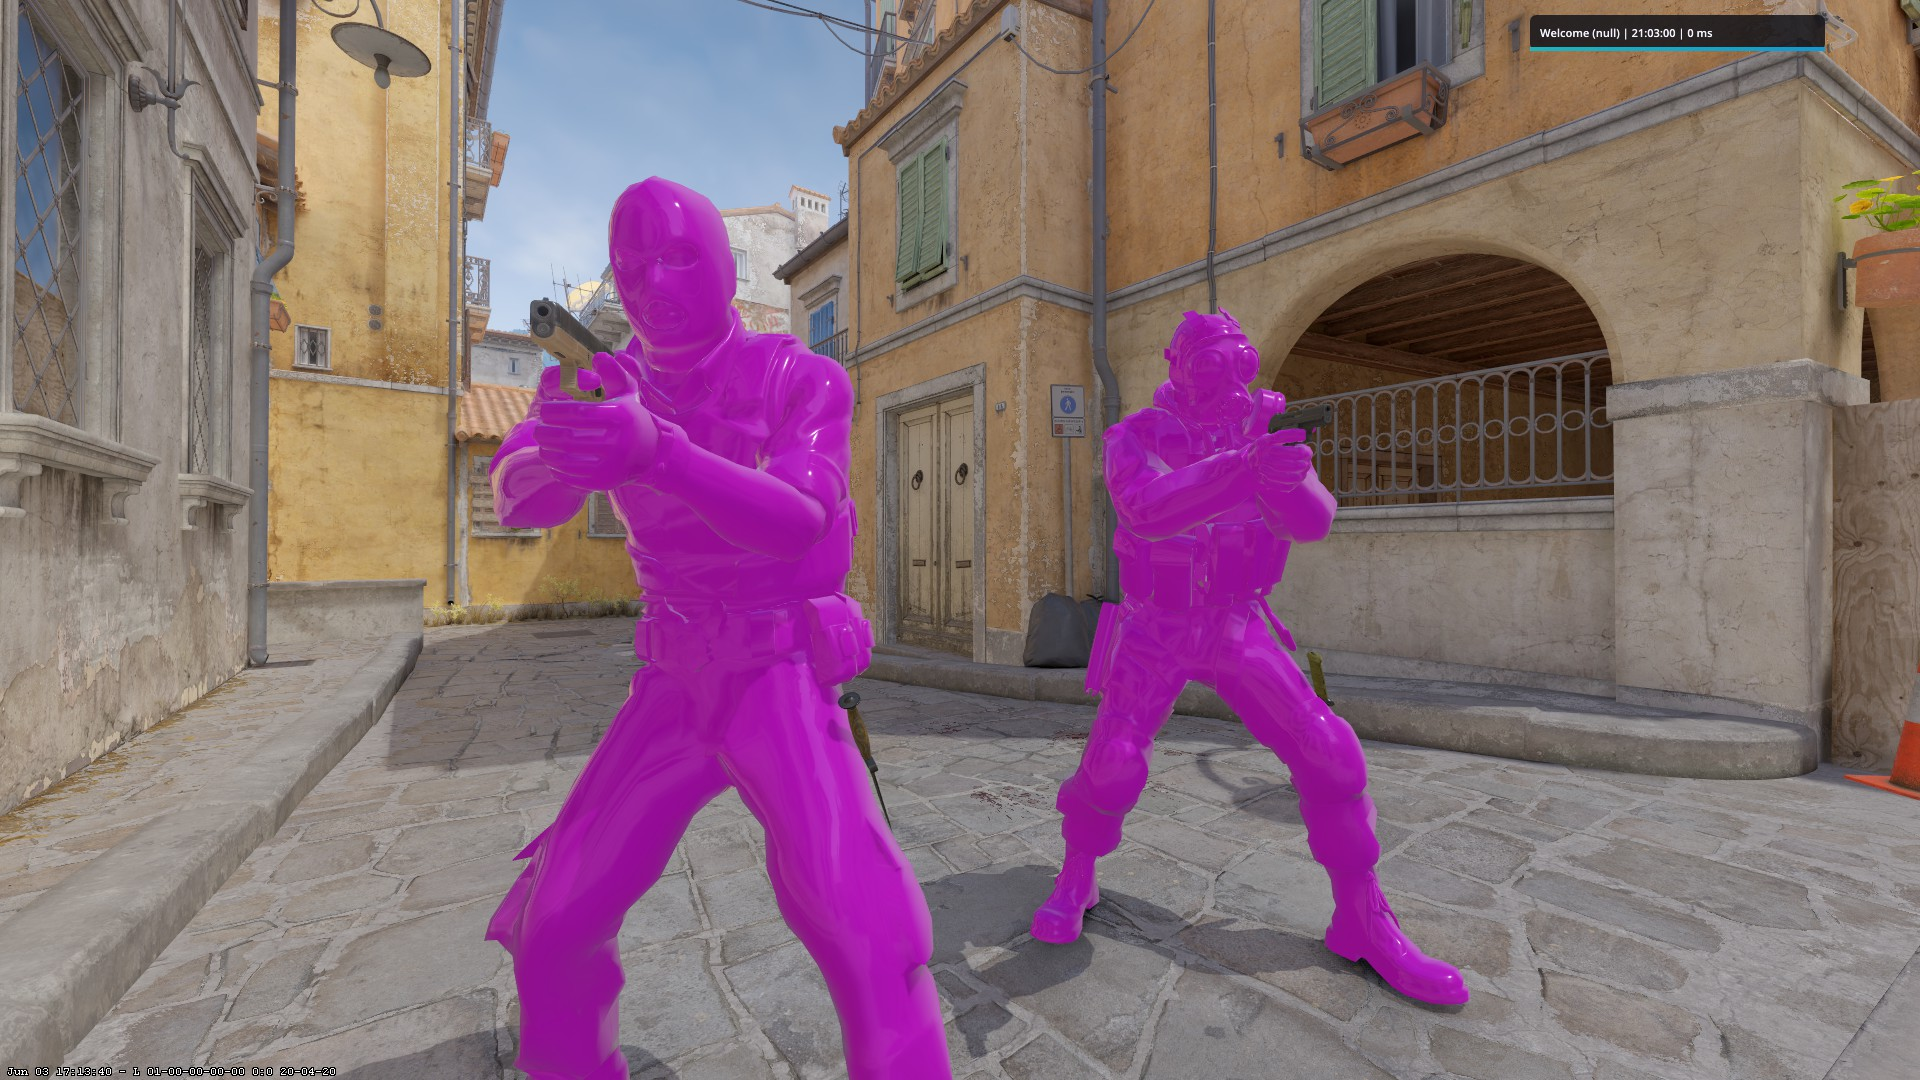
\includegraphics[width=1\linewidth]{../Master Thesis Template/images/chams/chams_demo/20250608210300_1.jpg}
\end{frame}

\begin{frame}
    \frametitle{Visual Examples: Chams Materials}        
    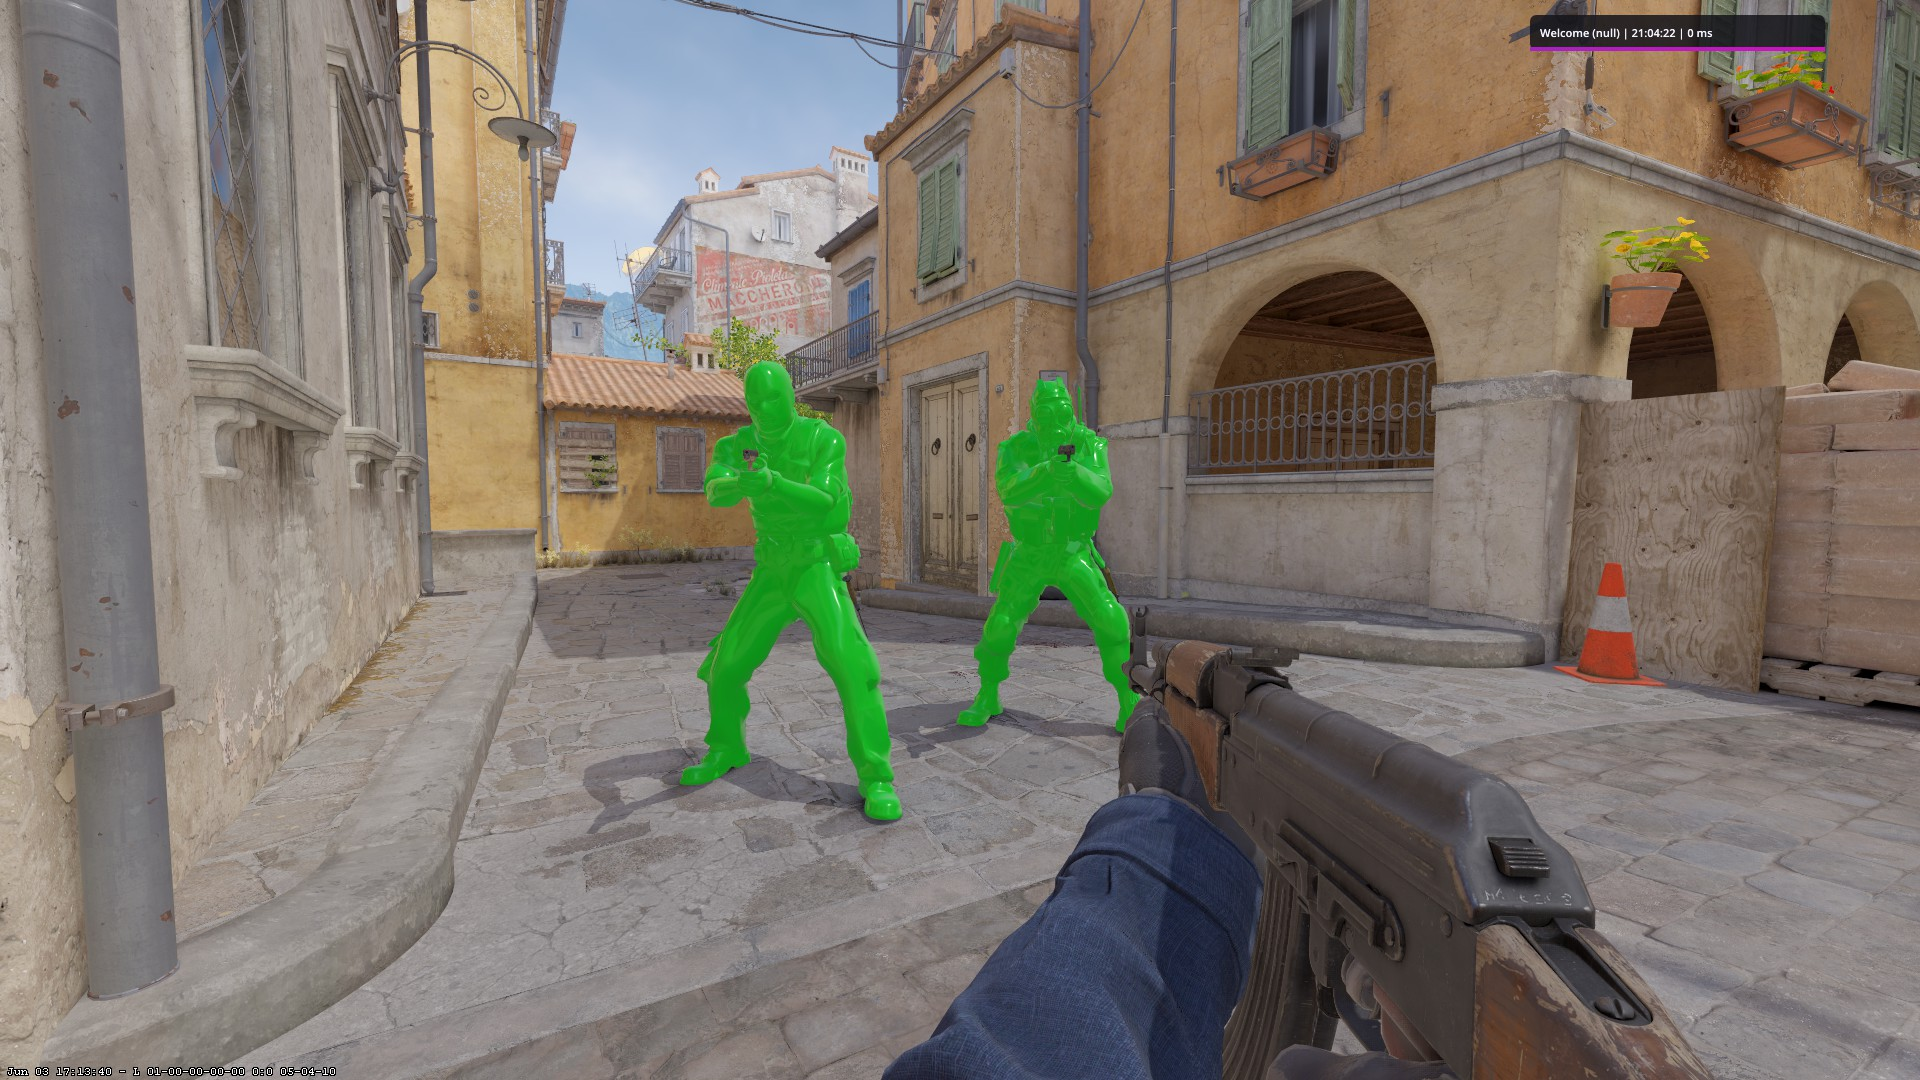
\includegraphics[width=1\linewidth]{../Master Thesis Template/images/chams/chams_demo/20250608210422_1.jpg}
\end{frame}

\begin{frame}
    \frametitle{Visual Examples: Chams Materials}        
    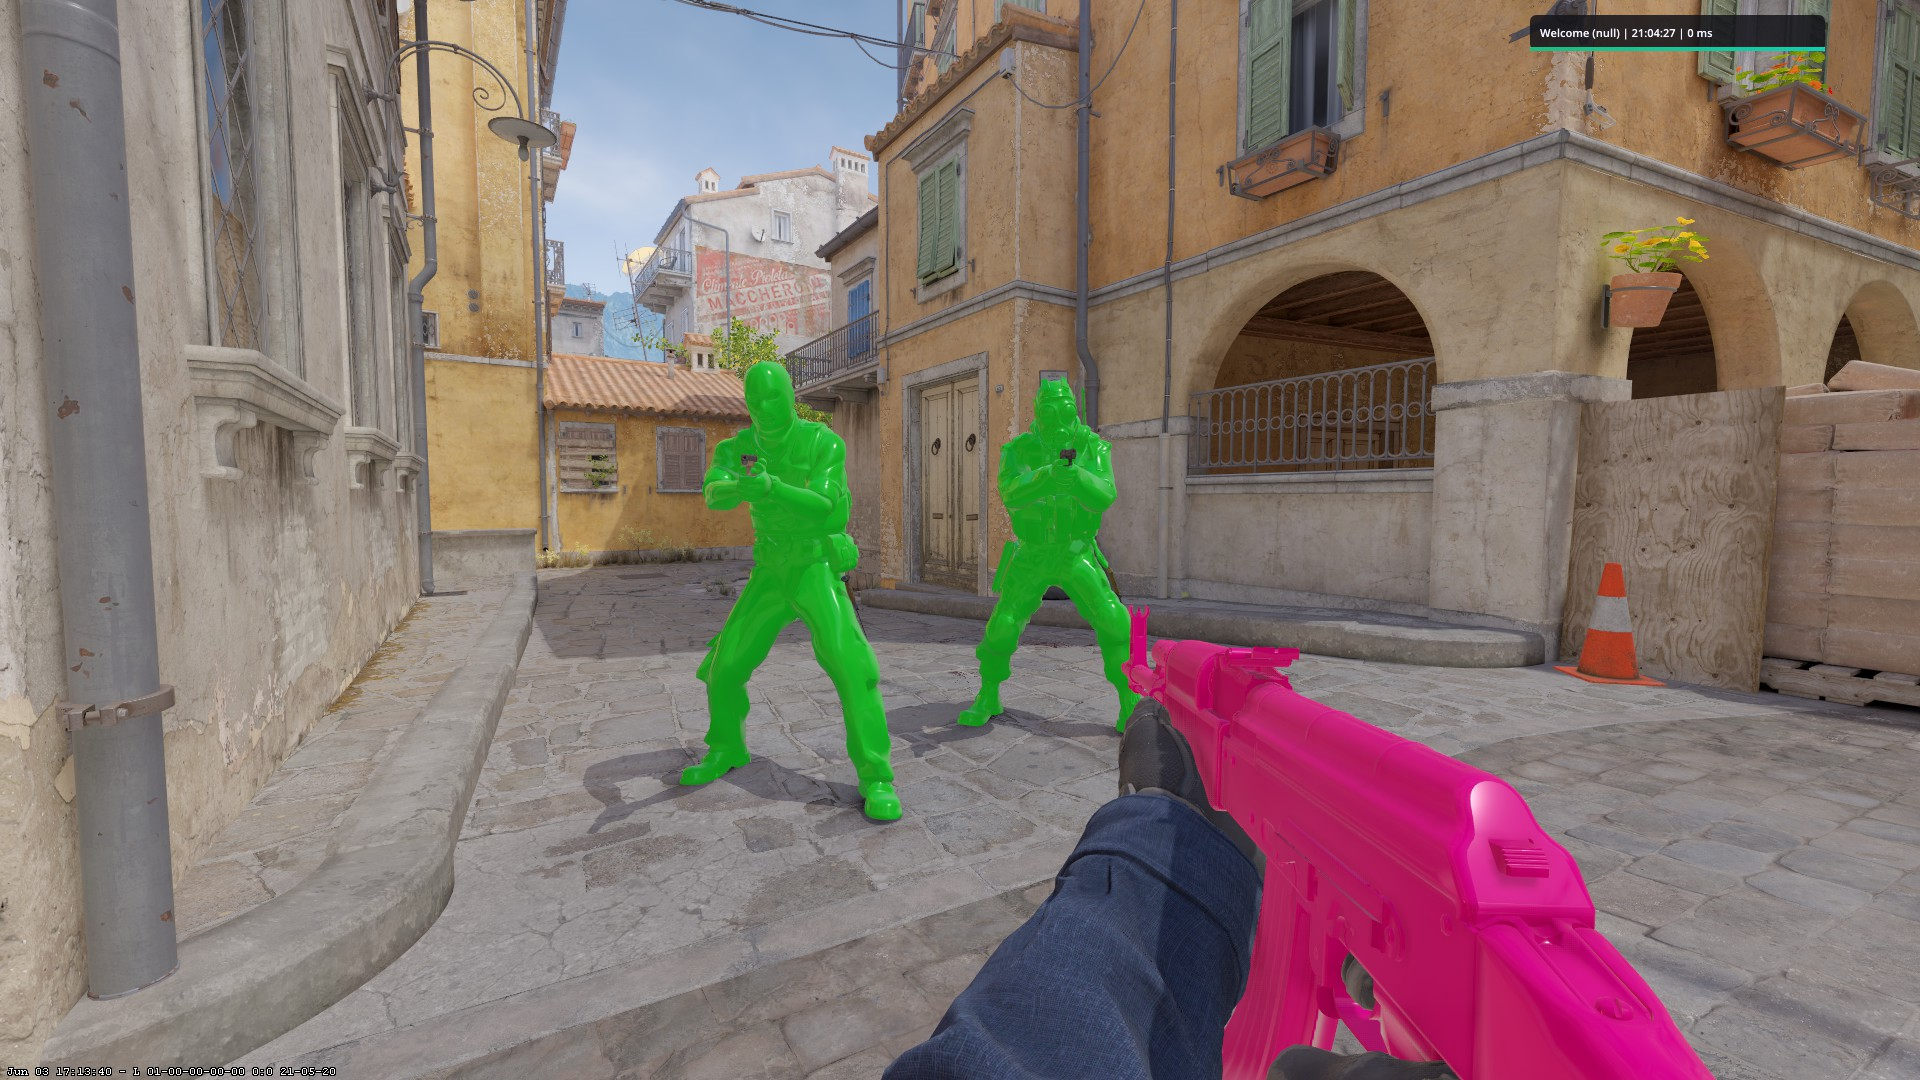
\includegraphics[width=1\linewidth]{../Master Thesis Template/images/chams/chams_demo/20250608210427_1.jpg}
\end{frame}



% --- NEW: Aimbot: Mathematical Overview ---
\begin{frame}
    \frametitle{Aimbot: Mathematical Overview}
    The aimbot determines the angle between the player and the target using 3D vector math.
    \vspace{0.4cm}
    \textbf{Angle Calculation:}
    \begin{equation*}
        \text{delta} = \text{targetPos} - \text{playerPos}
    \end{equation*}
    \begin{equation*}
        \text{yaw} = \text{atan2}(\text{delta}_y, \text{delta}_x) \times \frac{180}{\pi}
    \end{equation*}
    \begin{equation*}
        \text{pitch} = -\text{atan2}(\text{delta}_z, \sqrt{\text{delta}_x^2 + \text{delta}_y^2}) \times \frac{180}{\pi}
    \end{equation*}

    \vspace{0.4cm}
    \textbf{Explanation:}
    \begin{itemize}
        \item Converts a 3D vector into pitch and yaw angles required for aiming.
        \item Ensures consistent aiming regardless of relative position in space.
        \item Used each frame to update view angles if target is valid and visible.
    \end{itemize}
\end{frame}

% --- NEW: Aimbot: Target Selection and Smoothing ---
\begin{frame}
    \frametitle{Aimbot: Target Selection and Smoothing}
    For practical gameplay, raw angle calculation is insufficient. We enhance realism and precision using additional heuristics.
    \vspace{0.4cm}
    \begin{itemize}
        \item \textbf{Interpolation Factor:} We introduce a smoothing coefficient that linearly interpolates between the current view angle and the target angle, reducing abrupt snapping.
        \pause
        \item \textbf{Formula:}
        \[
            \text{newAngle} = (1 - \alpha) \cdot \text{currentAngle} + \alpha \cdot \text{targetAngle}
        \]
        where \( \alpha \in [0,1] \) controls the smoothing intensity.
        \pause
        \item \textbf{FOV Filter:} We filter potential targets by their distance to the center of the screen (Field of View), prioritizing those closer to the crosshair.
    \end{itemize}
\end{frame}


% --- NEW: Bone ESP: Skeleton Rendering via Bone Structures ---
\begin{frame}
    \frametitle{Bone ESP: Skeleton Rendering via Bone Structures}
    During our reverse engineering efforts, we located the in-memory structure used by CS2 to store bone positions for each player model.
    \vspace{0.4cm}
    \begin{itemize}
        \item \textbf{Bone Matrix Discovery:} The game maintains a matrix of bone positions indexed per entity, storing 3D coordinates for each joint.
        \pause
        \item \textbf{Rendering Strategy:} Once the matrix was located, we extracted the relevant joint coordinates and projected them into screen space.
        \pause
        \item \textbf{Skeleton Drawing:} We connected selected bones (e.g., head, spine, limbs) with lines to visually represent the player’s skeleton.
    \end{itemize}
\end{frame}


\begin{frame}
    \frametitle{Visual Examples: Bone Matrix}        
    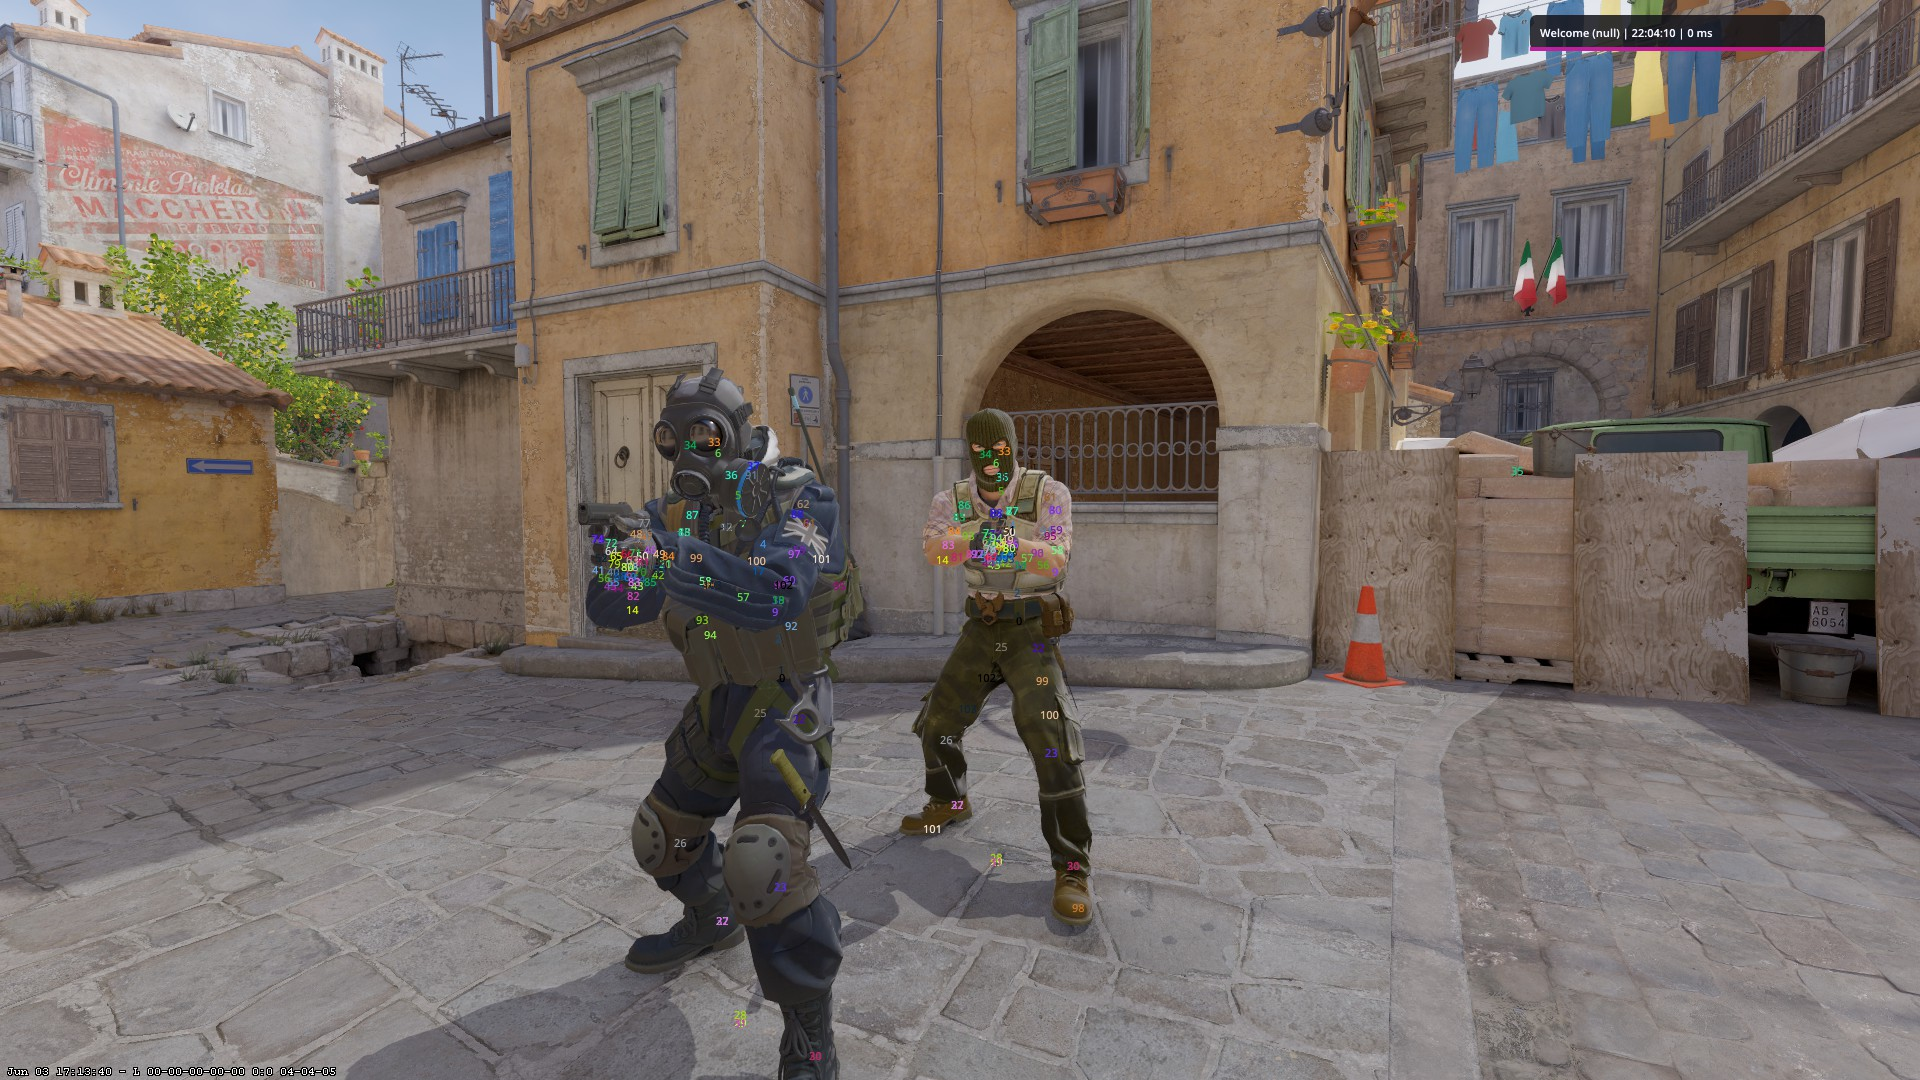
\includegraphics[width=1\linewidth]{../Master Thesis Template/images/Bones/20250608220410_1.jpg}
\end{frame}


\begin{frame}
    \frametitle{Visual Examples: Skeleton}        
    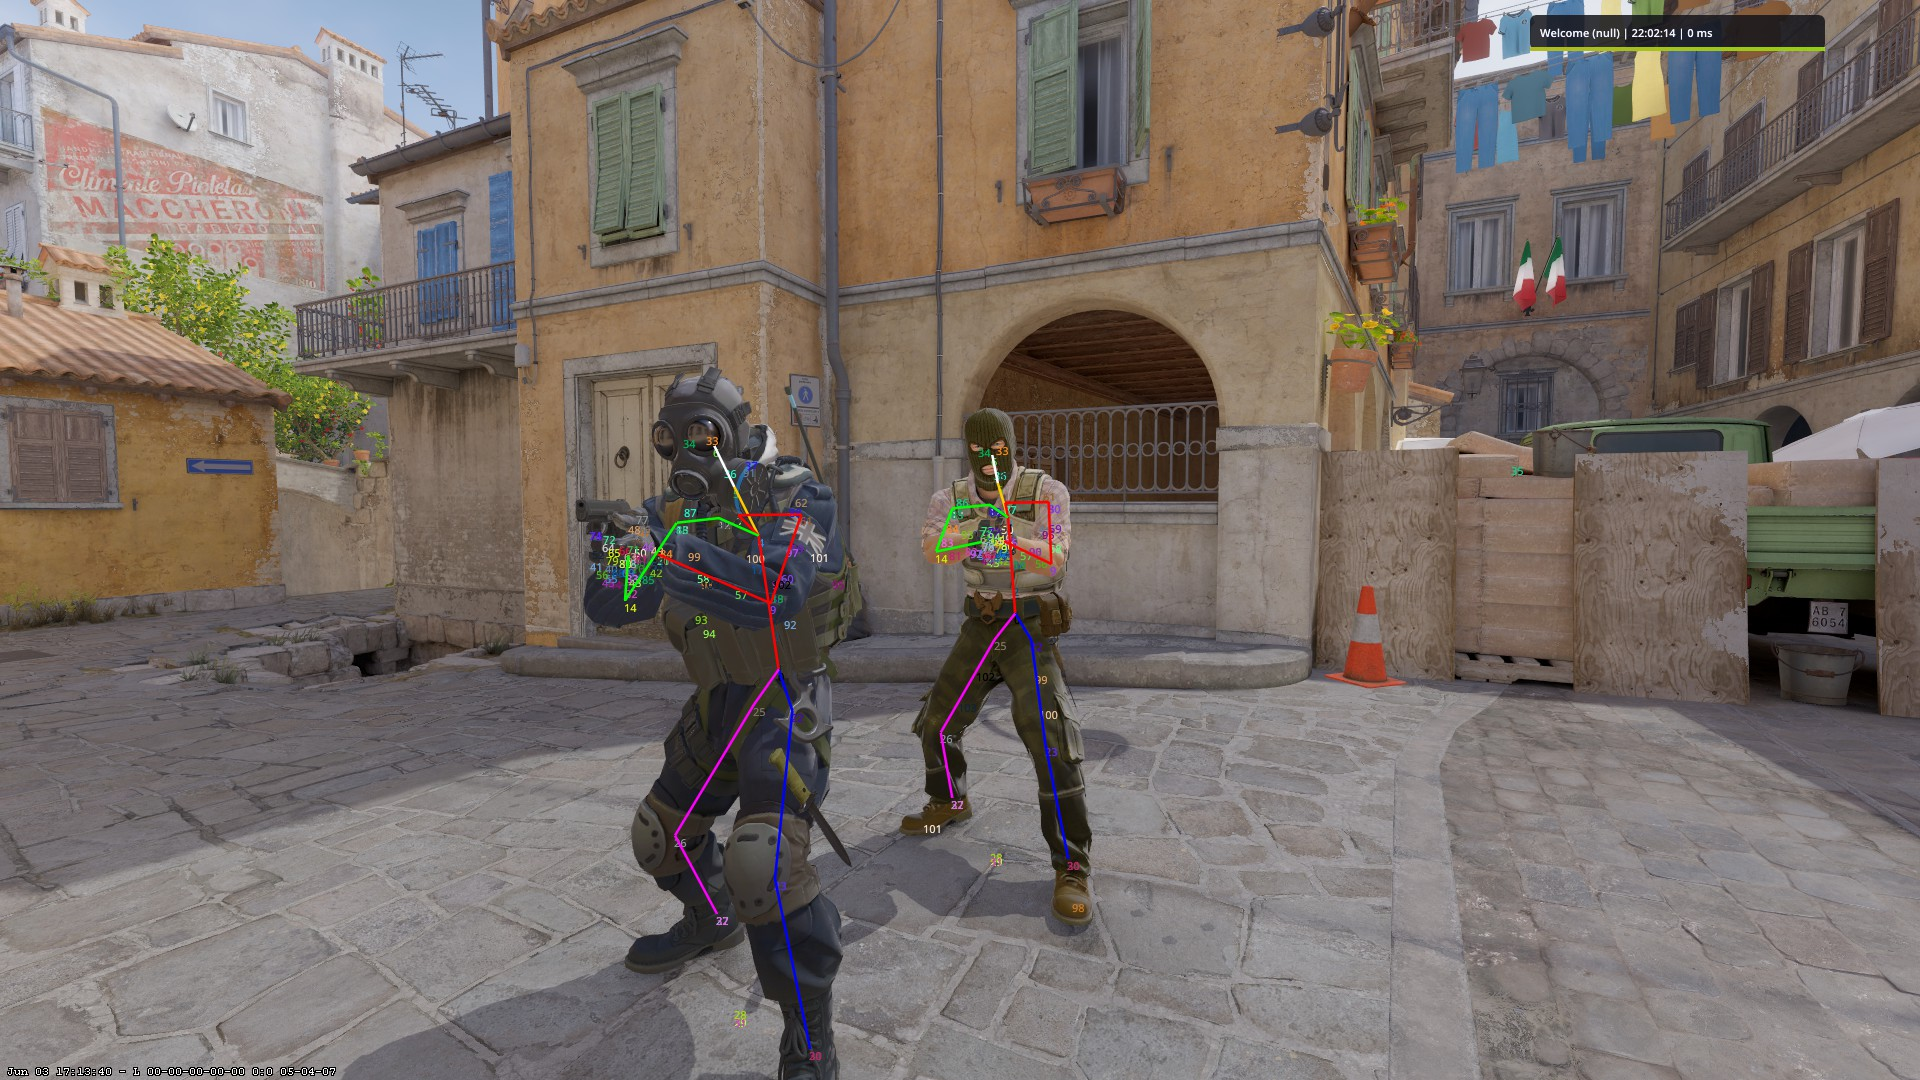
\includegraphics[width=1\linewidth]{../Master Thesis Template/images/Bones/20250608220214_1.jpg}
\end{frame}

\begin{frame}
    \frametitle{Visual Examples: Skeleton \& Chams in a Real Match}        
    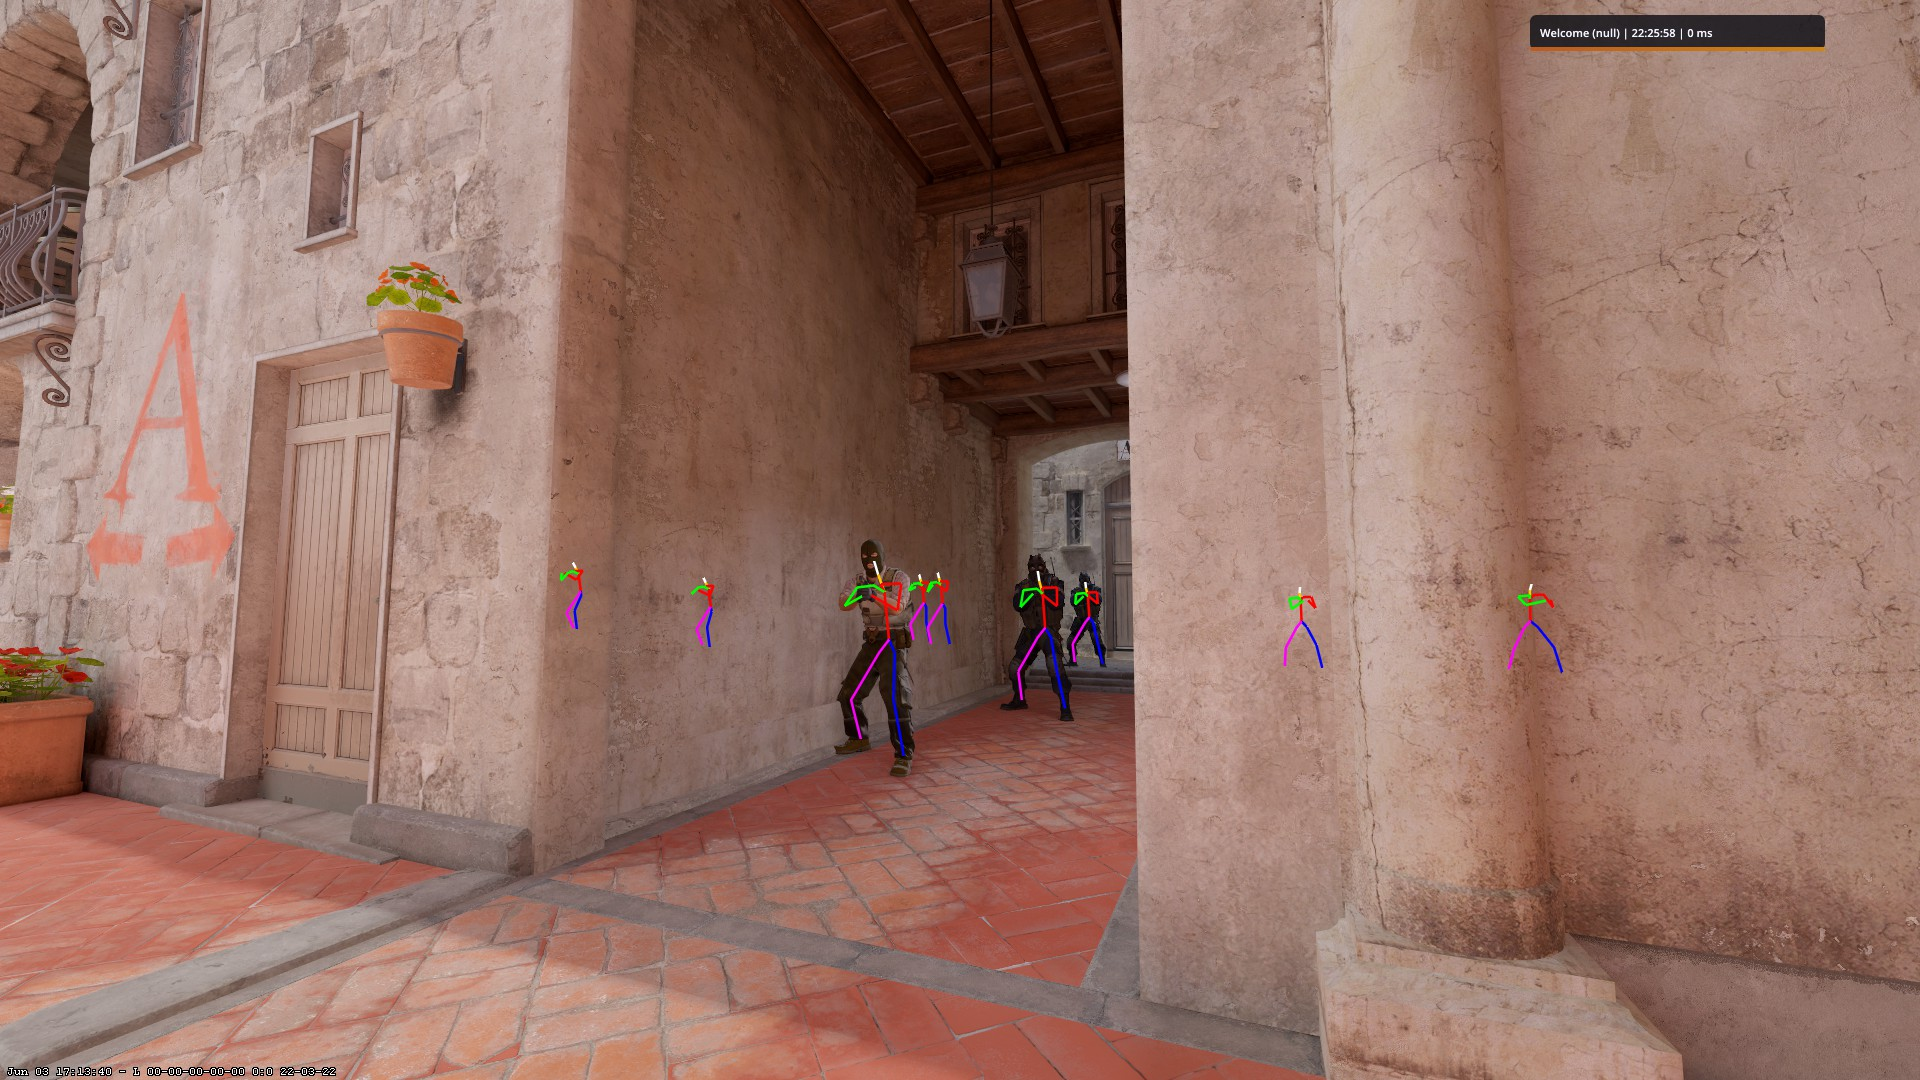
\includegraphics[width=1\linewidth]{../Master Thesis Template/images/Bones/20250608222558_1.jpg}
\end{frame}


\begin{frame}
    \frametitle{Visual Examples: Skeleton in a Real Match }        
    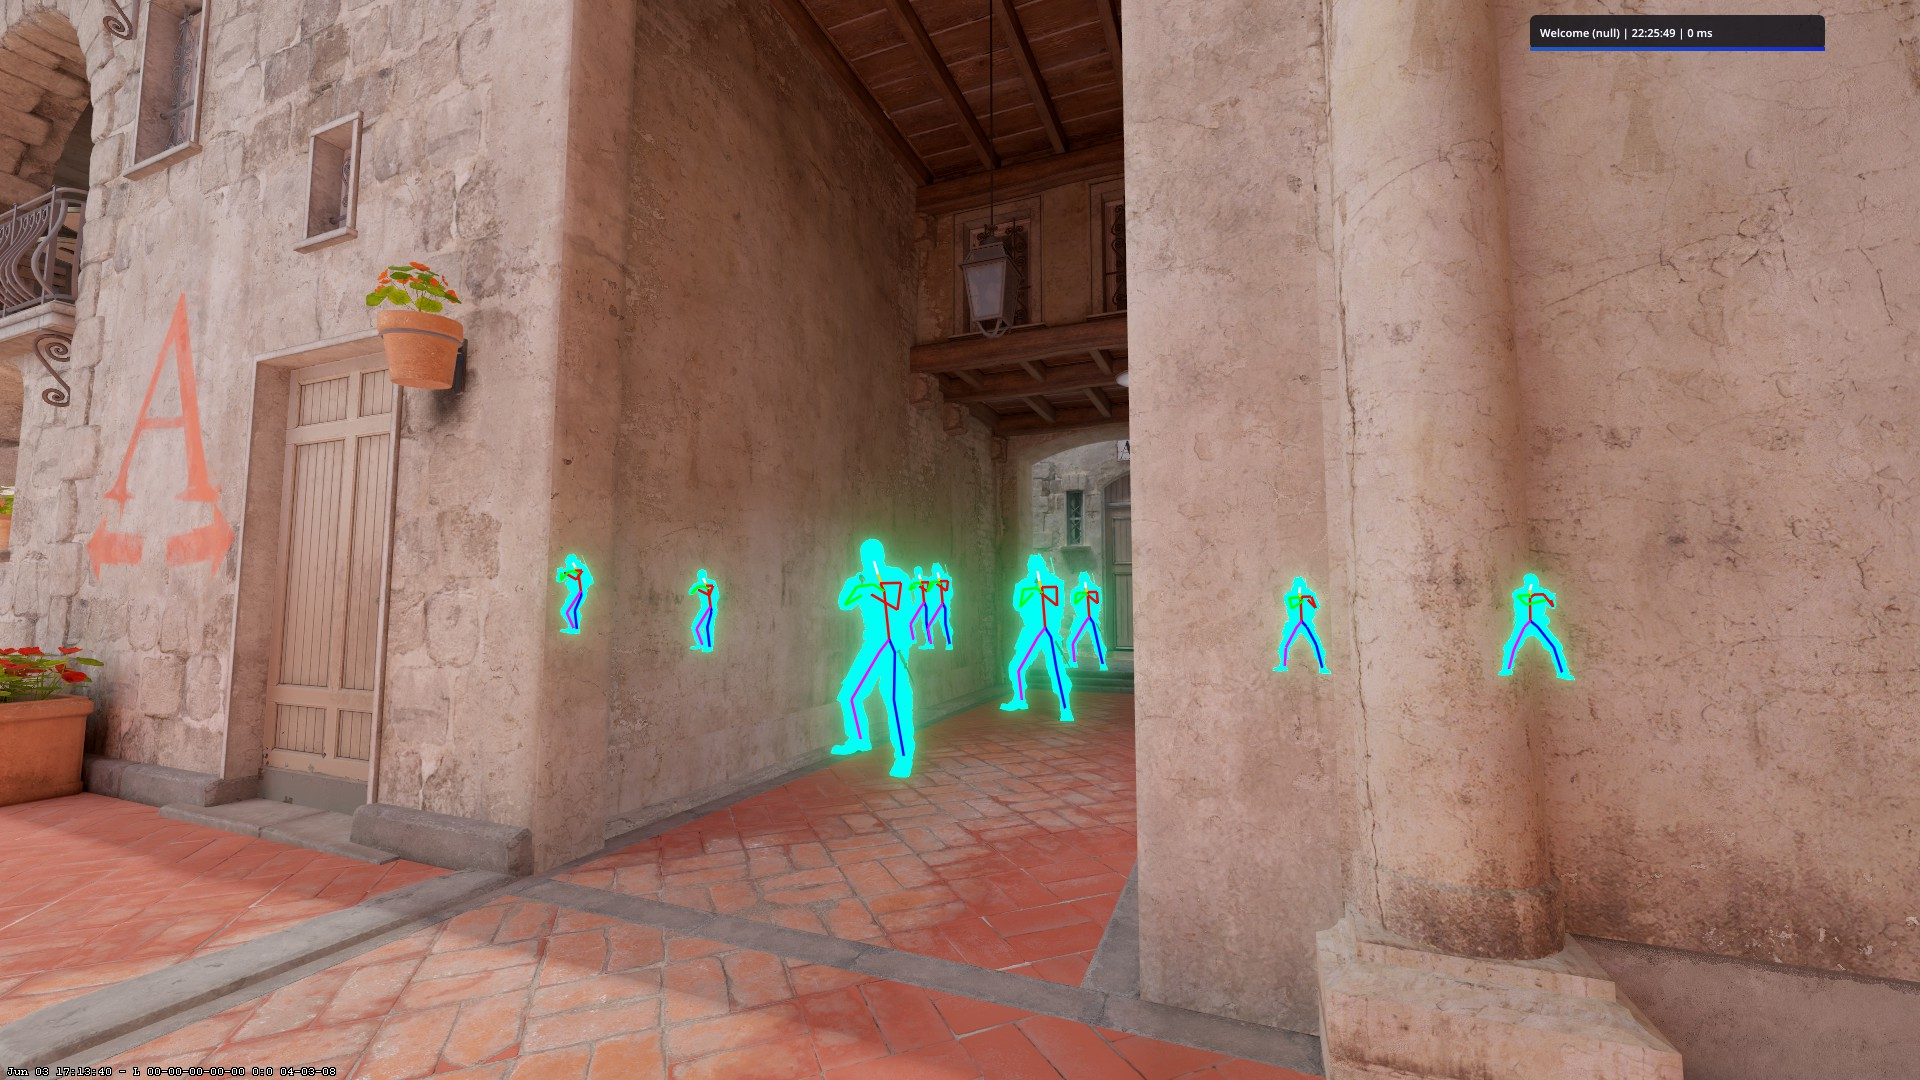
\includegraphics[width=1\linewidth]{../Master Thesis Template/images/Bones/20250608222549_1.jpg}
\end{frame}


\section{Reflections, Implications, and Future Work}

\begin{frame}
    \frametitle{Final Reflections}
    \begin{itemize}
        \item Cheating in online games reflects a complex interplay between technical ingenuity and social dynamics.
        \pause
        \item The continual arms race between cheat developers and anti-cheat systems mirrors broader cybersecurity challenges.
        \pause
        \item Gaining offensive insight through cheat implementation reveals critical blind spots in detection strategies.
        \pause
        \item Ethical, economic, and technical dimensions must be addressed together to preserve competitive integrity.
    \end{itemize}
\end{frame}

\begin{frame}
    \frametitle{Future Work and Research Directions}
    \begin{itemize}
        \item Extend the cheat framework to support multiple Source 2 titles, enabling comparative analysis.
        \pause
        \item Integrate automated schema extraction and dynamic offset resolution for update resilience.
        \pause
        \item Design and test new stealth hooking methods, including hardware breakpoints and kernel-level indirection.
        \pause
        \item Explore cheat detection benchmarking using controlled environments and real-time telemetry.
    \end{itemize}
\end{frame}


    

% --- Closing Questions Slide ---
\begin{frame}
    \frametitle{Questions}
    \begin{center}
        \Huge Thank you for your attention!\\[1em]
        \Large Any questions?
    \end{center}
\end{frame}

\end{document}
